\subsection{Infrastructure Reference Design}
\label{Sec:infraref}
Interferometric gravitational-wave detectors are large and complex devices and the selection of their site is an issue of great importance. The selected site should allow the highest possible level of scientific productivity at reasonable cost of construction and operation, and at minimal risk. Of paramount importance are the selection criteria that impact the scientific potential of the observatory. These include natural and anthropogenically generated environmental noise and site geological properties that affect construction cost.

Einstein Telescope will have excellent sensitivity over a wide frequency range starting at a few Hz up to a few kHz. Within the infrasound observation bandwidth (up to 20\,Hz) the scientific potential is affected directly by site location and the observatory infrastructure. Therefore, it is of paramount importance that the infrastructure reference design maximizes the scientific potential of the observatory. 
\begin{figure}[h!]
	\centering
		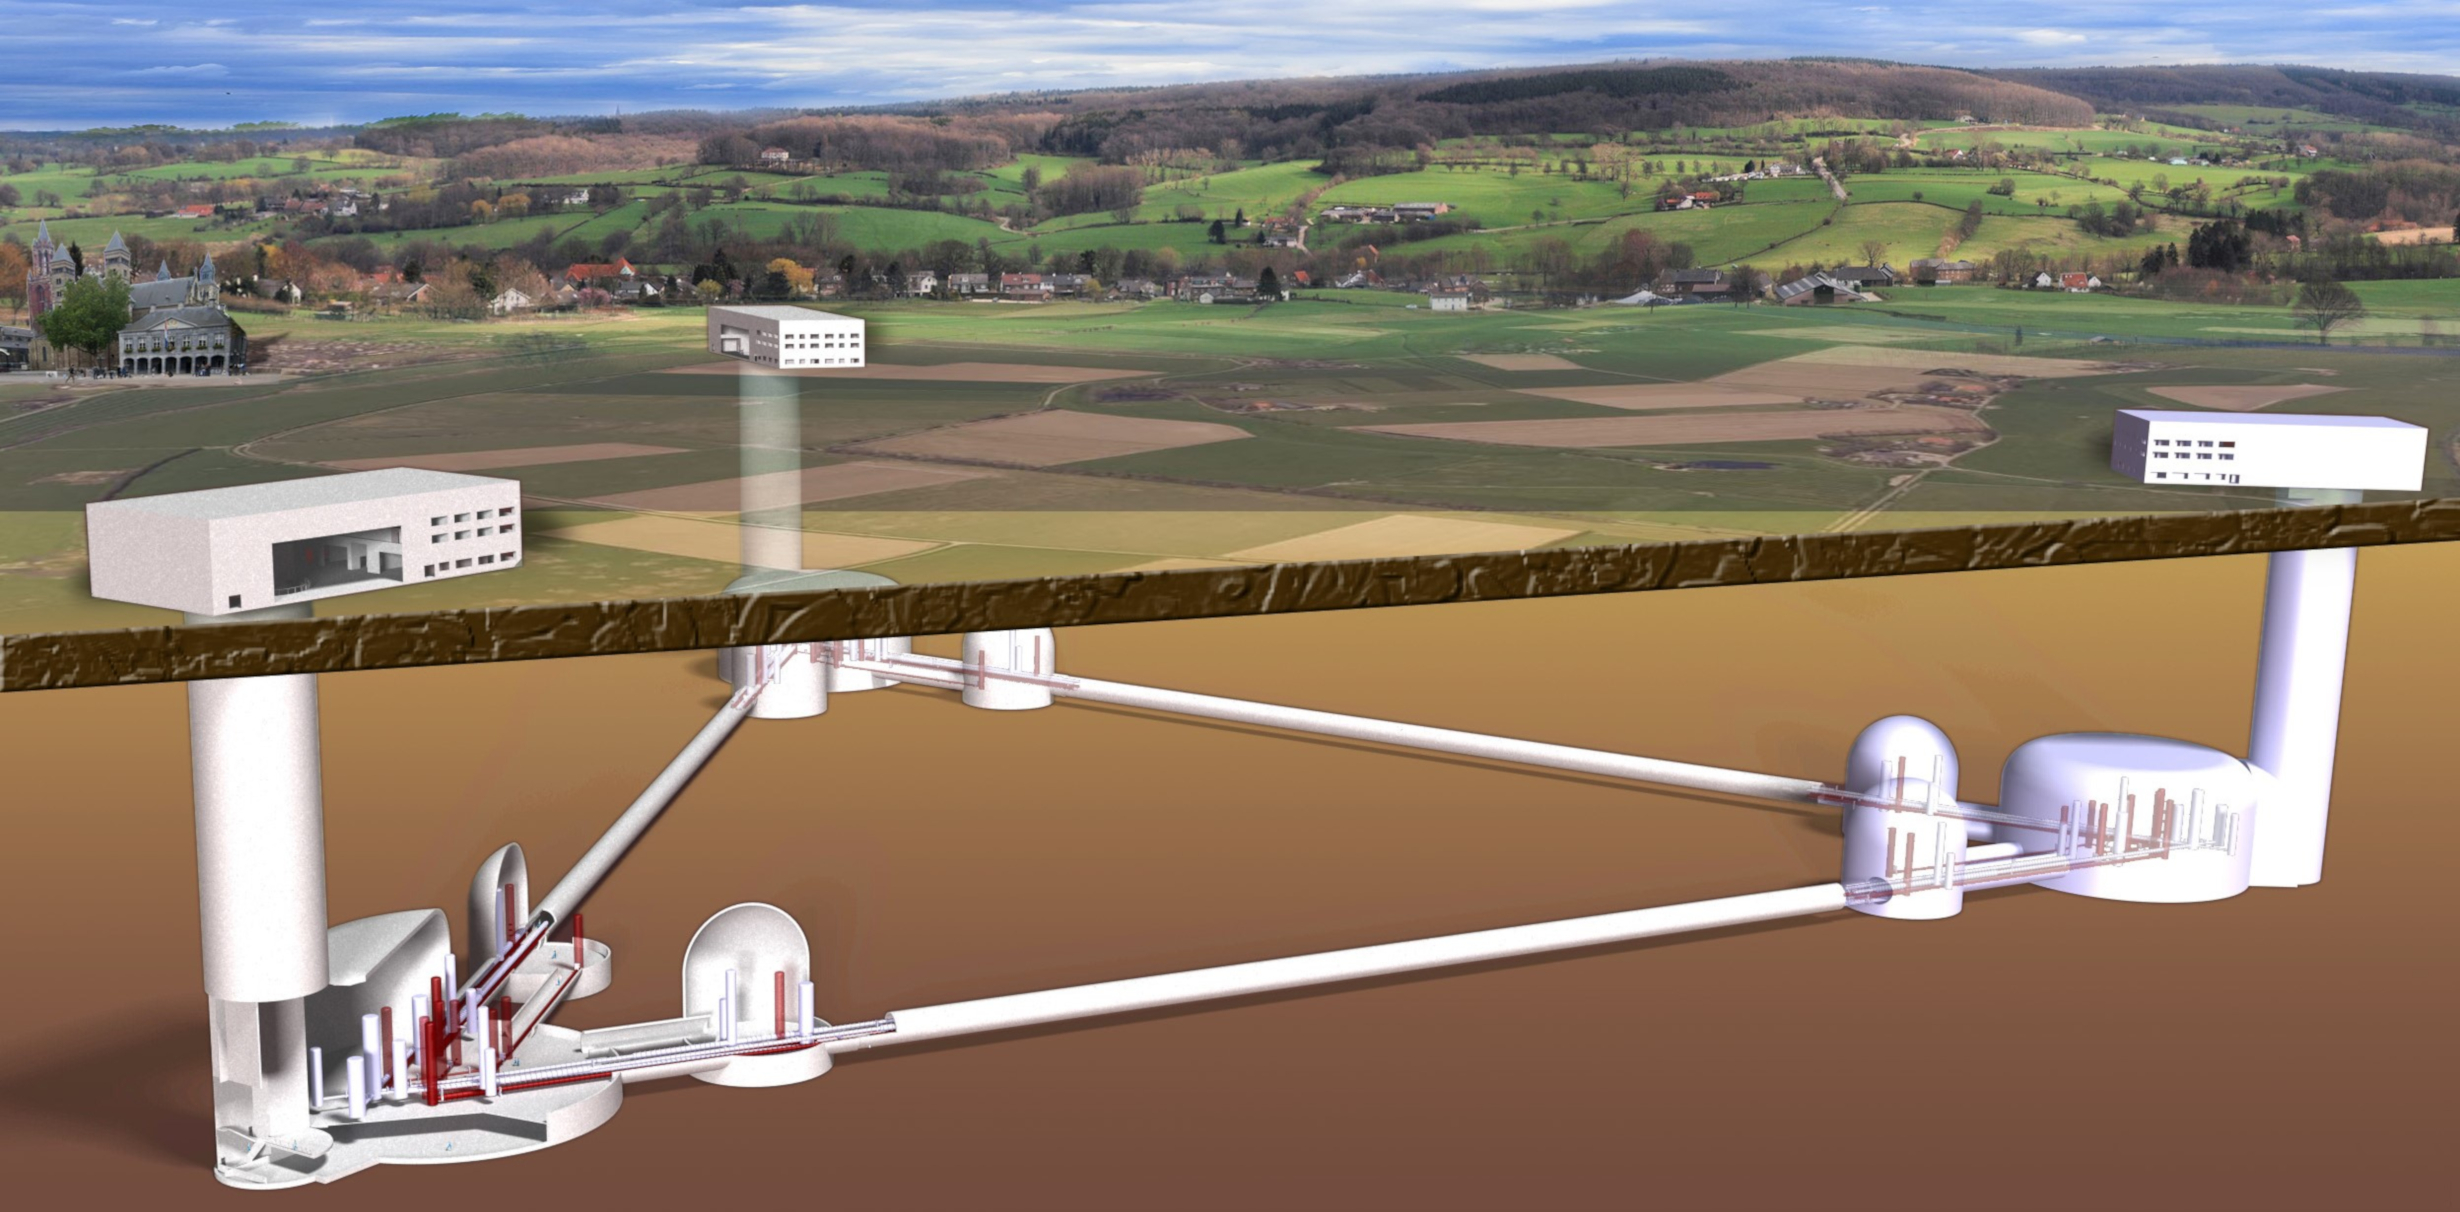
\includegraphics[width=\textwidth]{SiteInfra/SiteInfraFigures/ArtisticView2.jpg}
		\caption{Artistic impression of Einstein Telescope. The observatory has a triangular configuration that can house three xylophone detectors. Each detector is composed of a low-frequency cryogenic interferometer and a high-frequency interferometer operated at room temperature. The corner stations are connected by 10\,km long tunnels.}
		\label{Landscape}
\end{figure}

The local seismic activity is one of the most important site specific noise sources that can affect or degrade the interferometer performance. Mitigation of seismic displacement noise is achieved by combining careful siting with advanced suspension systems (outlined in section \ref{Sec:SASandSUS}). A prime example of a site that exhibits extremely low seismic background noise is the site selected for the Kagra detector in Japan. Kagra is located in the Kamioka mine, which currently holds the Super-Kamiokande experiment and the prototype cryogenic gravitational-wave detector, CLIO. The Kamioka facility is a former zinc and gold mine and is situated 250\,km west of Tokyo. Access to the underground facilities is through a well maintained horizontal road tunnel, allowing for depths down to 1000\,m. The performance requirements for Einstein Telescope will surpass those of Kagra and require that the infrastructure reference design advocates for a subterranean observatory. 

Among all sites that were studied as part of the Conceptual Design Study of the Einstein Telescope, two candidate sites remain and are currently under investigation: a site at the three-border region of Belgium-Germany-Netherlands, and another site at Sardinia near the former Sos Enattos mine. The main results of these investigations will be on the site conditions such as geology, geohydrology, accessibility, as well as on the characterization of environmental noise of natural and anthropogenic origin.

\subsection{Site conditions}
In this section, we describe the site-evaluation parameters (SEP) from an infrastructural and geological point of view. This should include all the possible parameters that have an impact on the excavation costs and construction timeline, detector operation, underground facility access convenience, safety of the workers in the underground environment and detector lifetime that we assume to be > 50 years.
The main goal of the site-selection and site-characterization process, the optimization of the layout of the facility (element of so-called “basic design”) and applied construction methods is the fulfillment of professional requirements of basic function, long-term, effective and appropriate operability of the Einstein Telescope. The technical and cost aspects, nevertheless, can only be optimized together, as a result of a multi-component decision-making procedure, balancing among sensitivity, cost and technical risk analyses. The most reasonable solution for the selected site, the basic design and the planned construction methods should ensure optimization both for technical readiness and the overall costs (both for construction and operation phases) of the facility. 
In the following, we give a list (to be completed) of parameters that should be considered, we group them in four categories i.e. surface, underground, safety and lifetime. The separation sometimes can be fictitious because the parameters can have an impact on more than one category. 

\paragraph{Surface} This section includes all the parameters related to the area where the detector is located and its surroundings. All collected data will be the starting point for the construction of a dedicated GIS (Geographic Information System). We divide the surface parameters in Construction, Support Infrastructures, Operation and Risk. For the Construction it is required an analysis of the surface conditions that includes: 
\begin{itemize}
\item	Collection of updated numerical maps and geodatabase 
\item	Extraction of updated orthophotos and 3D digital surface model (1:2000)
\item	Analysis of crustal deformation and ground stability (DInSAR analysis, etc)
\item	Geological surveys
\item	Geomorphological analysis
\item	Land use, parks and protected areas, hazard maps
\item	Hydrography of the region
\item	Main and secondary road networks and their typical load
\item	Existing technological networks in the area (power, gas, data, water supply, sewage systems)
\item	Presence and classification of wells and water uptake systems
\item	Site availability and acquisition costs
\item	Analysis of access portals including safety access along arms
\item	Environmental restrictions (waste control especially with respect to rock disposal, water control, soil conservation, nature and landscape conservation, environmental impact)
\item	Legal issues must be considered for what concerns the authorization procedures and the analysis of territorial constraints.
\item	Local labor costs
For the Support Infrastructures we identify the following parameters:
\item	Site accessibility 
\item	Accommodations for resident staff (housing, schools, shopping, etc.) 
\item	Accommodations for visiting staff (hotels, transportation, etc.)
\item	Local technical support (qualified vendors, maintenance, fabrication, etc.)
\item	Site utilities installation (power, water, etc.)
The factors that can affect the detector Operation are:
\item	Climate (wind speeds, precipitation, lightning rate)
\item	Cost of power
\item	Heating and cooling requirements of underground caverns (in combination with humidity control)
\item	Maintenance requirements
\item	Travel time and costs for visiting staff
\item	Cost of living
Among the Risks for the construction of the ET detector we must consider:
\item	Environmental risks (earthquakes, floods, windstorms) 
\item	Potential future anthropogenic noise from regional development including windfarms, rail service, manufacturing industry; agreements with local authorities should be made to minimize the risk that anthropogenic environmental noise increases during the lifetime of the Einstein Telescope that may cause its observation capabilities to be degraded
\end{itemize}

\paragraph{Underground}  The parameters related to the underground have been grouped in Rock Mechanics, Groundwater, Seismicity. The general aim of Rock Mechanical data acquisition is understanding and forecasting the real behavior of host rock mass, the variability of the parameters/processes/phenomena (as a function of rock types, weathering level, parting, lateral and vertical position, anisotropy, etc.) in order to reduce the uncertainties of input data of static design and ensure the technical/economic optimization of the facility. Preliminary geophysical study (mainly 2D and 3D seismic methods) must determine the positions of dislocations and faults and also the rock inhomogeneity. Parameters to be considered are:
\begin{itemize}
\item	Position of dislocations and faults
\item	Rock mass classification
\item	Strength parameters (uniaxial and triaxial compressive strength, tensile strength, shear strength of intact rocks and discontinuities)
\item	Elastic parameters (Lame-constant, Young-modulus, Poisson-ratio, compression and shear modulus, P-wave modulus)
\item	Anelastic parameters (relaxation times, other rheological parameters, etc…)
\item	Constitutive model of rock(s)
\item	Distribution of rock stresses
\end{itemize}

On the base of the rock classification, we can define a feasibility matrix for the ET detector obtained using 3D numerical modeling, which is shown in Figure \ref{tab:rockclass}. The grading of the underground elements are coded as 3=feasible, 2=hard, 1=challenging, 0=extremely hard. In the matrix are considered both the triangular (modified compared to the ET conceptual design for what concerns the main caverns size) and L-shape configuration.
\begin{figure}[h!]
	\centering
		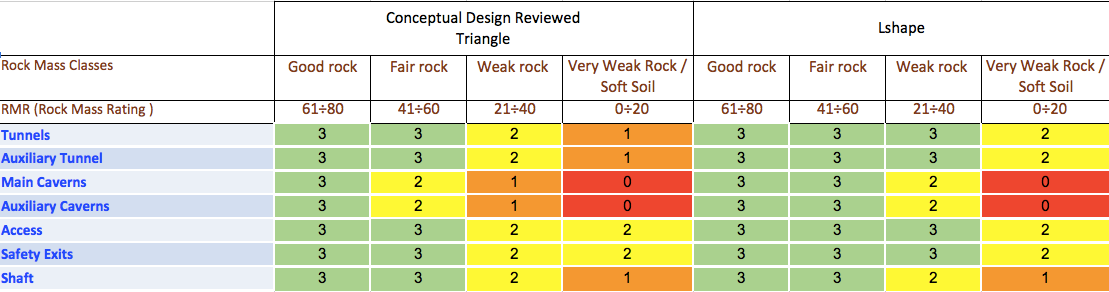
\includegraphics[width=\textwidth]{SiteInfra/SiteInfraFigures/RockClassTable.png}
		\caption{Feasibility of ET underground elements as function of rock classification.}
		\label{tab:rockclass}
\end{figure}
For what concerns the Groundwater, hydrogeological data must be collected corresponding to the different lithological faces (i.e. nature of the geological formations) that can be potentially encountered.  Hydraulic conductivity is the most important parameter to assess the quantity of groundwater to be potentially drained by underground galleries and cavities. As hydraulic conductivity in hardened rocks is highly dependent on the faulting, local degree of fractures, interconnectivity and apertures must be considered. Another big issue is certainly the depth-dependent values for hydraulic conductivity in a given lithology. It means that extrapolation of observed values is not easy and in situ deep borehole hydraulic tests are needed. In karstic limestones, the hydrogeological parameters are quite heterogeneous with local variation of several orders of magnitude in hydraulic conductivity added to a lack of ‘representativity’ of most of the field and borehole in situ tests and measurements. It means that the acquired values from future field tests would be processed with care and that conservative assumptions would be needed for all future hydraulic and stability calculations. The main hydrological parameters to be considered are:
\begin{itemize}
\item	Hydraulic conductivity
\item	Porosity
\item	Effective drainage porosity
\item	Dispersivity coefficients
\item	Water table position 
\item	Water table amount/size
\end{itemize}

\paragraph{Seismicity} A specific aspect of the seismicity in relation to the site geology is the Seismic Microzonation. We can have variations of seismic-noise amplitude at small scales due to filtering, damping, and amplification. Filtering is the frequency-dependent transmission of seismic waves, for example, through stratified geology. Amplification under “stable conditions” is the effect of the interference of seismic waves trapped within geological bodies bounded by large seismic impedance contrasts (soft soil/bedrock, soil/free surface, etc.) irrespective of the absolute impedance values. The dimension of geological bodies and discontinuities to be analyzed for characterizing the relevant phenomena are of the order of the seismic wavelengths. Damping is related to soil and rock properties in terms of a material’s quality factor, but it can also be a consequence of scattering from small-scale, geological heterogeneities. All these effects are potentially important for the design of a Newtonian-noise cancellation system. 

\paragraph{Safety}  A parameter to be considered for the safety of the workers at the detector site is the Radioactivity. The primary radioactive elements in the Earth’s crust that lead to human exposure are potassium, uranium, thorium, and their radioactive decay products (e.g. radium, radon). The majority of the dose to the lung arises from exposure to the short-lived decay products of radon and thoron. Radon and thoron are ubiquitous in the air at ground level and are significant contributors to the average dose from natural background sources of radiation. In homes, in underground mines and in other situations where radon (and thoron) may be present and where ventilation may be limited, the levels of these radionuclides and their decay products can accumulate to unacceptably high levels. Soils and rocks are often the main sources of radon. In unsaturated soils or rocks, radon moves in gaseous form through pores and fractures. In saturated zones, radon moves in solution into groundwater to underground openings, such as mines and caves, and to buildings. For underground facilities it is important to consider the contribution from the outdoor environment through the ventilation system and from building materials. While most building materials produce small amounts of radon, certain materials can act as significant sources of indoor radon. Such materials have a combination of elevated levels of 226Ra (the radioactive parent of radon) and a porosity that allows the radon gas to escape. Examples are lightweight concrete with alum shale, phosphogypsum and Italian tuff. EURATOM establishes reference levels for indoor radon concentrations and for indoor gamma radiation emitted from building materials. Recent epidemiological findings from residential studies demonstrate a statistically significant increase of lung cancer risk from prolonged exposure to indoor radon at levels of the order of 100 Bq m-3. 
Another risk element to be considered is the risk of Water Inrush during detector construction or operation.  An evaluation of the water-table size and position (see Groundwater section) and rock dislocations needs to be considered in order to evaluate the risk of flooding of the underground detector facility.

\paragraph{Lifetime}  The project should foresee for the ET infrastructure a lifetime longer than 50 years (as happens for all the big infrastructures). Parameters to be considered in this respect are:
\begin{itemize}
\item	Long-term ground stability; differential movements of rock masses due to, e.g., subsidence or shear zones over the extent of the Einstein Telescope need to be sufficiently small 
\item	Average and peak humidity in the caverns and along the tunnels
\item	pH of the groundwater and of the condensation over the facility structures
\item	Chemical elements (in particular chloride if stainless steel will be used for the pipes)
\item	Microbiologically Influenced Corrosion
\item	AC-induced corrosion due to nearby high-voltage electric power lines, railways etc.
\end{itemize}

\subsection{Environmental noise}
\label{sec:envnoise}

\FloatBarrier
\subsubsection{Seismic noise}
\label{SeismicNoise}
Noise studies \cite{Gutenberg1958, Asten1984, Peck2008} often categorize seismic noise sources according to frequency. For the Einstein Telescope, critical frequency regions are in the range of 0.1 -- 1\,Hz, where the seismic noise is variable mainly due to oceanic microseisms, and 1\,Hz and 10\,Hz, where seismic noise is dominated by local sources including human activity. Oceanic microseisms are connected to large-scale meteorological conditions at oceans, seas or large lakes. Significant anthropogenic noise has been observed at the existing detector sites from trains, road traffic, planes, logging operations, and above all, from the detector infrastructure including pumps and ventilation systems.
 \begin{figure}[h!]
	\begin{center}
		 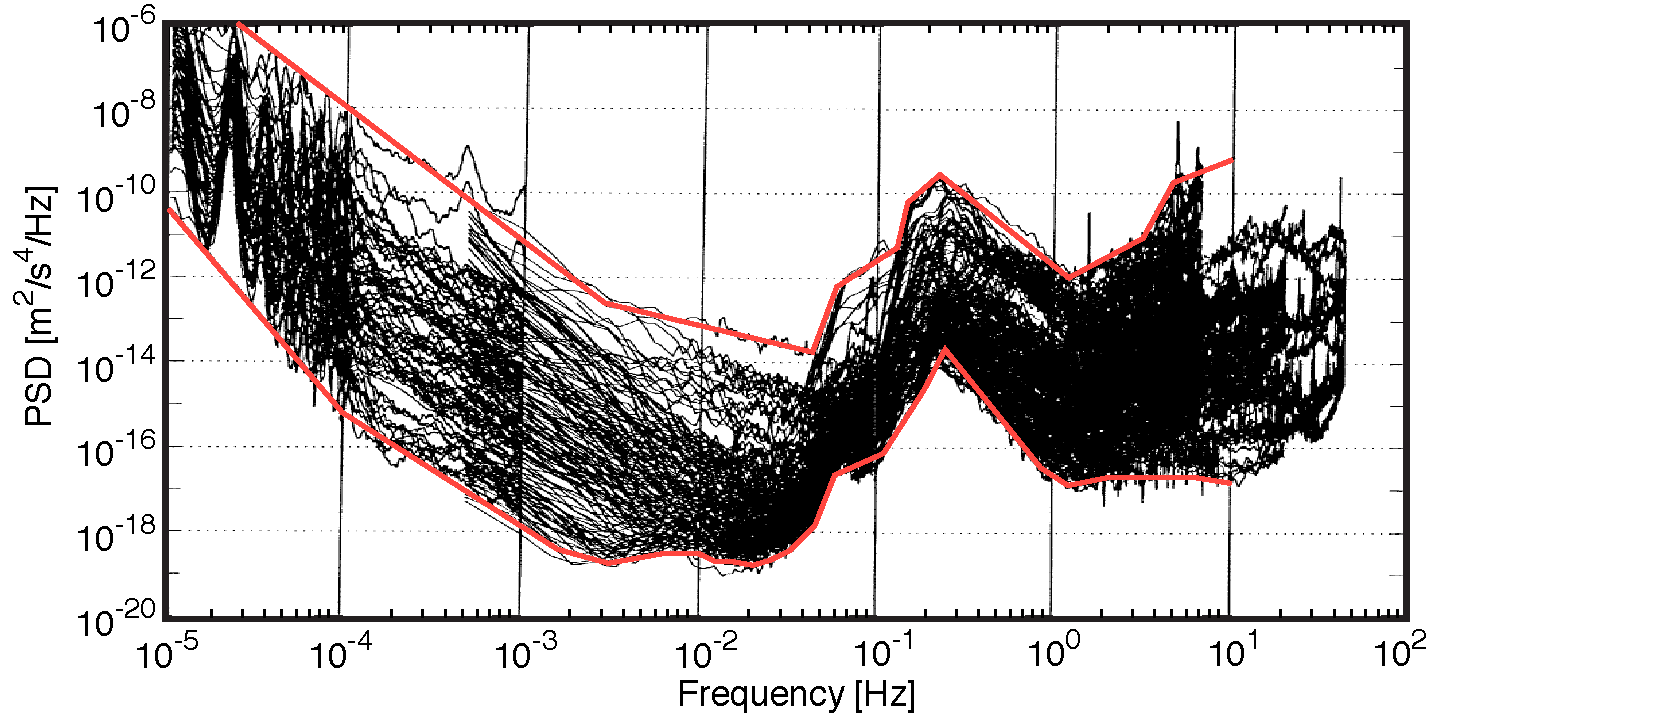
\includegraphics[width=\textwidth]{./SiteInfra/SiteRequirements/SiteRequirementsFigures/peterson2.pdf}
			\caption{Overlay of network station spectra used in Peterson's background noise study \cite{Peterson1993} together with straight-line segments fitted to the high-noise and low-noise envelopes of the overlay.}	
			\label{fig:peterson}
	\end{center}
\end{figure}

Seismic spectra are represented as power spectral densities (PSDs) as shown in Fig. \ref{fig:peterson}. The largest PSD values are seen at low frequencies. Here, the surface of the Earth experiences large external forces due to the gravitational attractions of the Moon and Sun. At very low frequencies this causes the surface of the Earth to rise and fall with amplitudes of about 0.5\,m with respect to the center of the Earth. This tidal motion can be seen in Fig. \ref{fig:peterson} at a frequency of $2.3 \times 10^{-5}$\,Hz. Since the motion occurs at very low frequency, the interferometer test masses will move {\sl coherently} and differential test-mass motion presents no problem. Large PSD values are also observed at frequency around $5 \times 10^{-2}$\,Hz and 0.2\,Hz, which correspond to oceanic microseisms. 

Peterson \cite{Peterson1993} catalogued acceleration noise power spectral density plots for frequencies up to 50\,Hz from 75 seismic stations distributed worldwide. Several years of data were collected (about 12,000 spectra in total). From the upper and lower bound of the combined data of both surface and borehole sensors (100 - 340\,m depth) Peterson derived, what is now known as, the new high/low noise model (NHNM/NLNM). The data including the upper and lower bound fit are shown in Fig. \ref{fig:peterson}. 

Presently, the large interferometric detectors GEO600, LIGO, and Virgo are placed on the surface of the earth and, consequently, are sensitive to seismic disturbances. Figure \ref{fig:groundsites} shows a comparison of seismic acceleration power spectral densities of the GEO, KAGRA, Virgo, and LIGO Hanford and Livingston sites. From these ground motion measurements it is clear that the level of seismic noise reduction in the underground environment of KAGRA is less stringent by several orders of magnitude. \tcr{This plot might indeed be useful, but it was not included in the CDR files actually...} The seismic attenuation system of the Einstein Telescope as described in section \ref{Sec:SAS} will be able to suppress ground motion by many orders of magnitude down to about a Hz, thus opening the low-frequency window below 10\,Hz to GW observations.

As explained, the NLNM is a composite of many different stations and instruments with different geology and in various geographic regions. Therefore, it is not possible to observe this spectrum at one specific location. Lowest noise in the 10\,mHz to 10\,Hz band is typically obtained at remote continental sites far from oceans and human activity, and with predominantly hard-rock geology. Generally, low seismic noise is also observed in boreholes and inactive mines. Highest quality surface sites as well as underground sites can have PSDs that lie only by a small factor above the NLNM.

\paragraph{Anthropogenically generated seismic noise}
The influence of traffic induced seismicity on GW detectors has been studied by various authors. Road noise depends on road structure and materials, traffic density and vehicle type and speed. Schofield $et$ $al.$ \cite{Schofield2000} reported that local traffic from passenger vehicles to heavy trucks induced vibrations at the LIGO Hanford, WA, site. Vibrations were measured for frequencies in the 1 -- 50\,Hz range, with maxima around 4 - 12 Hz. At the Virgo site, road noise was analyzed by using recordings of the seismic field at the Virgo site and correlating these recordings with measurements underneath a major high way overpass, 4\,km away from the Virgo North arm terminal building~\cite{VIR-NOT-FIR-1390-251}. Seismic noise originating from the nearby traffic was found in frequency ranges of 1 -- 4\,Hz, peaking at 3\,Hz. Coward $et$ $al.$ \cite{Coward2003} recorded ground vibrations at the AIGO site in Australia for vehicles passing the instrumentation as close as 24\,m. Road noise was visible in the 5 -- 30\,Hz frequency band.

In addition, the infrastructure of current GW detectors is a major source of noise above about 10\,Hz \cite{CoEA2016a,CoEA2018a}. Excess noise due to infrastructure can in principle be avoided, for example, by placing fans and pumps on dampers. Such measures are currently under investigation to lower infrastructure noise at the Virgo site. Thorne \emph{et al.} investigated how the interferometer is affected by noise originating from humans, animals, airplanes, etc.~\cite{GGthorneWinstein}. Within the subterranean environment this extends to placement of electricity generators, pumps, and cryo-coolers to keep the facility operational. These devices will be sources of seismic noise. Nonetheless, it is of great importance to avoid excess noise at the underground site of the Einstein Telescope since one could otherwise spoil the advantage of underground construction.

\paragraph{Wind generated seismic noise}
Wind noise has been studied by a number of authors to quantify the conversion of wind energy into ground motion \cite{WiEA1996,DABo2012}. The presence of wind causes movement of surface objects, such as trees or structures. It can exert turbulent pressures on topographic irregularities, and also the transport of an atmospheric pressure field with gradients by wind produces ground motion. Of particular interest for ET are the frequency characteristics of the wind noise, the wind speed threshold for it to become evident, and its persistence with depth. Most of the wind-driven sources of seismic noise predominantly produce local surface displacement and tilt. Only a fraction of this perturbation is associated with seismic waves, and the energy going into seismic waves is mostly associated with surface Rayleigh waves. Only a small fraction of wind noise propagates away from the surface. The reduction in wind noise is a prime example that surface seismic noise contributions will decay with depth. 

\subsubsection*{Terrestrial gravity noise}
Environmental disturbances are often associated with mass-density fluctuations, which can couple through gravitational attraction with the test masses. Sources of terrestrial gravity noise, also known as Newtonian noise (NN), include seismic and atmospheric fields as well as vibrating infrastructure and moving objects \cite{Har2015}. As will be explained in Section \ref{sec:depthNN}, mitigation of NN is the strongest argument to construct the Einstein Telescope underground. It would be an immense, potentially impossible task to design a NN mitigation system (see Section \ref{Sec:NewtonianNoise}) that would provide the same noise reduction at the surface. It is most difficult to model NN from the ambient seismic and atmospheric fields described in the following two sections, which have therefore enjoyed the greatest attention so far. As potentially important sources of these fields, it is important to anticipate the effect of noisy infrastructure and to present low-noise infrastructure designs. Acoustic and seismic fields at the LIGO and Virgo sites are currently dominated by infrastructure noise.

\subsubsection*{Seismic gravity noise}
Seismic NN is a complex composition of different effects, which means that a detailed understanding of the seismic field is required to model the seismic NN, and to predict the performance of a cancellation system if required. Seismic fields can change mass density in two ways: either they cause (de)compression of the soil and rock, or they displace interfaces between materials of different density or surfaces of materials. The two surfaces to be considered in all modeling problems are Earth's surface and the walls of underground caverns.

Seismic fields are generally a composition of several wave types including the Rayleigh waves, which are surface waves, and compressional and shear waves, which are longitudinally and transversely polarized body waves that can travel in any direction through a medium \cite{AkRi2009}. Since some of the seismic sources can be part of the detector infrastructure, one also needs to understand the properties of near fields of sources. Generally, a precise prediction of NN is only possible taking all properties of the seismic field into account including propagation directions, polarizations, location of sources, and scattering of seismic waves. Such detailed understanding can be obtained with extensive surface and underground seismometer arrays, and potentially also with a combination of limited seismic measurements and numerical simulations if detailed knowledge of geology, topography, and location of seismic sources is available. 

Past observations in underground environments demonstrated that seismic fields have a high level of stationarity \cite{CoEA2014,BaEA2017}, but there are only few published results of the stationarity of underground seismic fields, and it is conceivable that average distributions of seismic sources change over long periods of time, and even rock properties might change for example due to varying water content. Such details might become important for the design of NN cancellation systems, which is why site-characterization studies should foresee a long-term underground seismic measurement.

\subsubsection*{Atmospheric gravity noise}
Atmospheric perturbations can produce noise in GW detectors in two ways. Either they are the cause of vibrations of components of the detector, or they produce NN, which is a consequence of direct gravitational coupling between test masses and environmental disturbances. Acoustic NN can have contributions from the atmosphere, but also from the caverns that host the test masses of the Einstein Telescope \cite{FiEA2018, Har2015}. In the last case, infrastructure sources become relevant. Since a noise-cancellation system (see Section \ref{Sec:NewtonianNoise}) is easier to design for cavern NN due to the absence of wind, the main challenge is to understand the atmospheric NN and to be able to predict how it is reduced by going underground.

The properties of the atmosphere give rise to many possible mechanisms to produce NN. Generally, one can associate atmospheric gravity fluctuations with fields of pressure, temperature, or humidity. It is often useful to categorize atmospheric processes according to a characteristic length scale describing the phenomena: global scale, synoptic scale (several 100\,km to several 1000\,km), mesoscale (several 1\,km to several 100\,km), and the microscale (up to several 1\,km). Mostly the microscale phenomena are relevant to NN modeling in GW detectors. Mesoscale phenomena might become relevant at frequencies below a few 10\,mHz, i.e., below the Brunt-V\"ais\"al\"a frequency. One source of gravity perturbations are microscale pressure fluctuations in the planetary or atmospheric boundary layer \cite{Ell1972a,McHe1975}, which is the lowest part of the atmosphere directly influenced by the surface. They can be divided into static and dynamic pressure fluctuations. Static pressure fluctuations, which include sound, are present even in the absence of wind \cite{AlEA1998}, while dynamic pressure fluctuations are connected to anything that requires wind \cite{BMS2004,ScJe2018}. There is also a connection between the two, for example, through the Lighthill process, which describes the generation of sound waves by turbulence \cite{Lig1952,Lig1954}. Additional structures emerge with the presence of wind such as vortices or so-called coherent structures \cite{TrEA2015}. 

Atmospheric gravity perturbations have been known since long to produce noise in gravimeter data \cite{Neu2010}, where they can be observed below a few mHz. Creighton published the first detailed analysis of atmospheric NN in large-scale GW detectors \cite{Cre2008}. It includes noise models for infrasound waves, quasi-static temperature fields advected in various modes past test masses, and shockwaves. Atmospheric gravity perturbations are expected to be the dominant contribution to ambient NN below 1\,Hz, and can still be significant at higher frequencies \cite{FiEA2018}. Generally, the Navier--Stokes equations need to be used to calculate density perturbations and associated gravity fluctuations \cite{Dav2004}. Quasi-static density perturbations associated with non-uniform temperature or humidity fields can be transported past a gravity sensor and cause gravity fluctuations. 

\subsubsection*{Considerations on detector depth}
\label{sec:depthNN}
A vacuum system and sophisticated seismic isolation provide the bare minimum of decoupling between a laser-interferometric GW detector and its environment. However, a few other coupling mechanisms cannot be avoided in this way including direct gravitational coupling between environment and test masses, and stray-light noise. Gravitational noise was described above. Stray-light noise is caused by a small fraction of light scattered out of the main laser beam due to imperfections of the optics' surfaces, then being reflected from a strongly oscillating surface, for example, of the vacuum chambers, and finally being reflected back towards the main laser beam, with which it partially recombines. Even though the overall efficiency of this scatter process is small, it is posing the currently dominant coupling between environment and interferometer in Virgo. It turns out that the stray-light noise is dominated by an up-conversion of high-amplitude, low-frequency vibrations of the reflecting surfaces \cite{CaEA2013}. It is suppressed by blocking the path of scattered light with absorbing baffles. Important here is that the low-frequency vibrations and therefore stray-light noise are not significantly suppressed by going underground since the vibrations are associated with oceanic microseisms, which travel as several kilometer long seismic waves. The Einstein Telescope is planned to be only a few 100\,m underground. 

Going underground is beneficial for seismic isolation. Specifically, ground tilts are known to be much stronger at the surface due to the direct impact of the atmosphere \cite{DABo2012}. The reduced tilt can make an important difference in active seismic isolation, where tilt-to-horizontal coupling in seismic sensors poses performance limitations \cite{MaEv2015,MLMa2018}. However, the implementation of tiltmeters in the active isolation systems \cite{VeEA2014} or more substantial redesigns of active seismic isolation platforms \cite{MLMa2018} are possible to mitigate the problem. Therefore, while reduced ground motion in underground environments is clearly beneficial for seismic isolation systems, it is not the most important aspect. 

The most important gain of going underground is to reduce terrestrial gravity noise. Atmospheric and seismic NN can both be reduced. Predicting the reduction of surface seismic NN with depth requires the dispersion curves of surface Rayleigh waves. The slower the medium, the shorter the waves, the stronger the suppression with depth. An example of the suppression factors as a function of frequency for various depths is shown in Figure \ref{fig:RayleighNNdepth}. 
\begin{figure}[t]
	\begin{center} 
		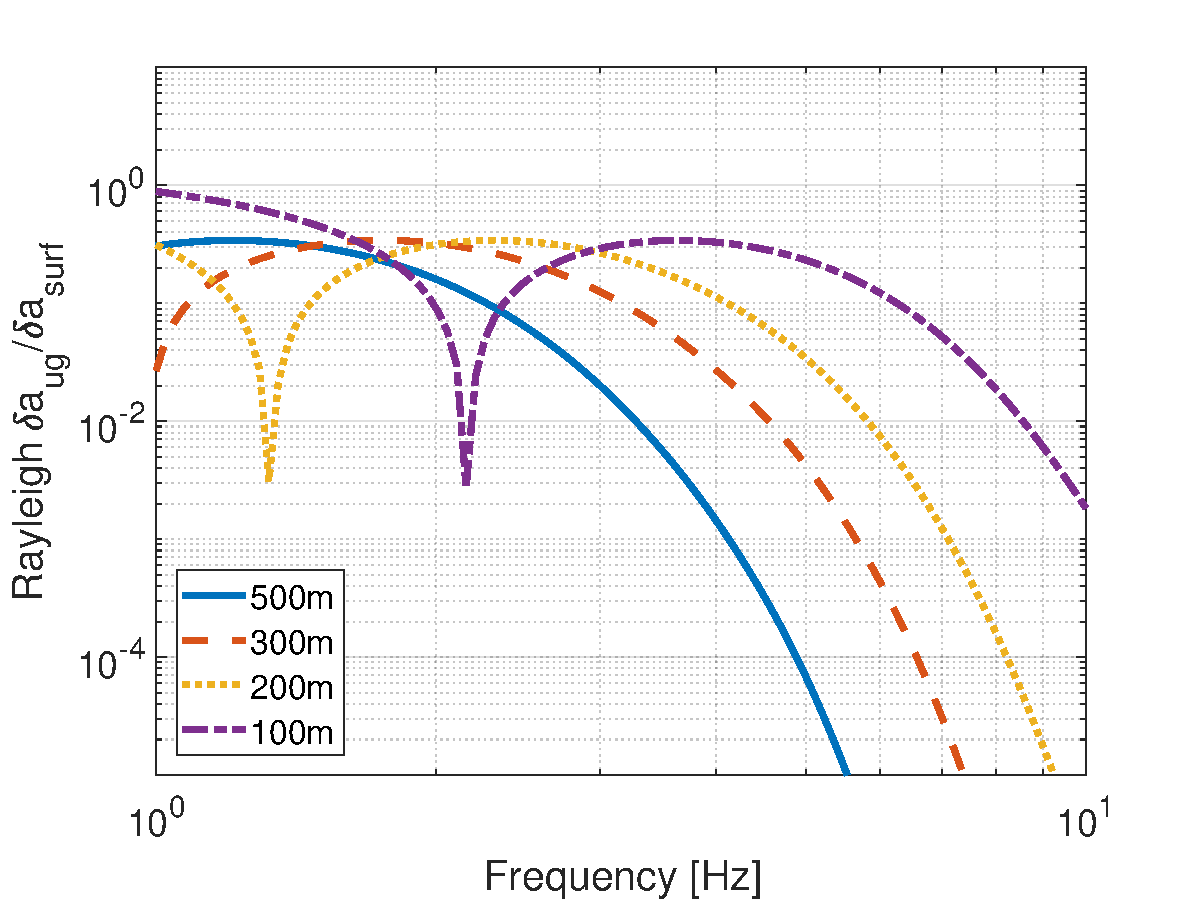
\includegraphics[width=0.7\textwidth]{./SiteInfra/SiteRequirements/SiteRequirementsFigures/RayleighNNdepth.pdf} 
		\caption{Suppression of Rayleigh-wave NN with depth. In this model, it is assumed that wave speed falls from 1.8\,km/s at 1\,Hz to 500\,m/s at 10\,Hz. These suppression curves are used in the right plot of Figure \ref{fig:NNestimates}.}
		\label{fig:RayleighNNdepth} 
	\end{center}
\end{figure}
Seismic speed is assumed to be 1.8\,km/s at 1\,Hz falling smoothly to 500\,m/s at 10\,Hz. Since the Einstein Telescope targets GW measurements down to a few Hz, it is clear if NN needs to be reduced by an order of magnitude and more (see Figure \ref{fig:NNestimates}), then a depth of 100\,m would not be sufficient in this example. Also relevant, but not shown here, is the reduction of atmospheric NN. Results presented in \cite{FiEA2018} showed that atmospheric, acoustic NN is expected to be sufficiently reduced already at 100\,m depth, and it is to be expected that all forms of atmospheric NN are sufficiently suppressed at such depth since the corresponding fields vary over much smaller distances compared to seismic fields, which is essential for the suppression of NN with depth. 

In conclusion, the most important gain of underground construction is the reduction of NN, and seismic NN is most relevant as it requires greater depths for strong reduction. Other important criteria affected by detector depth include the detector construction cost, safety regulations, and the required performance of a NN mitigation system. To choose the optimal detector depth, one needs to weigh the different aspects, which will generally depend on the site properties.







